\subsubsection{Các màn hình dành cho Host}
\label{sec:screen-host}
Kênh Host tổ chức tổng quan, không gian, booking, tin nhắn và tài khoản. Đơn xin quyền Host nằm tại \texttt{hostApplications/\{uid\}}, gồm thông tin liên hệ và hai ảnh giấy tờ DEMO; hồ sơ chỉ được cấp quyền khi Admin chấp thuận. Sau đó Host tạo tòa nhà, phòng và cấu hình cho thuê. Hình~\ref{fig:actual-host-editor} minh họa danh sách tòa nhà và biểu mẫu đăng phòng; dữ liệu được gửi qua HostViewModel tới HostRepository.

\begin{figure}[!htbp]\centering
\begin{minipage}[t]{0.40\linewidth}\centering\vspace{0pt}
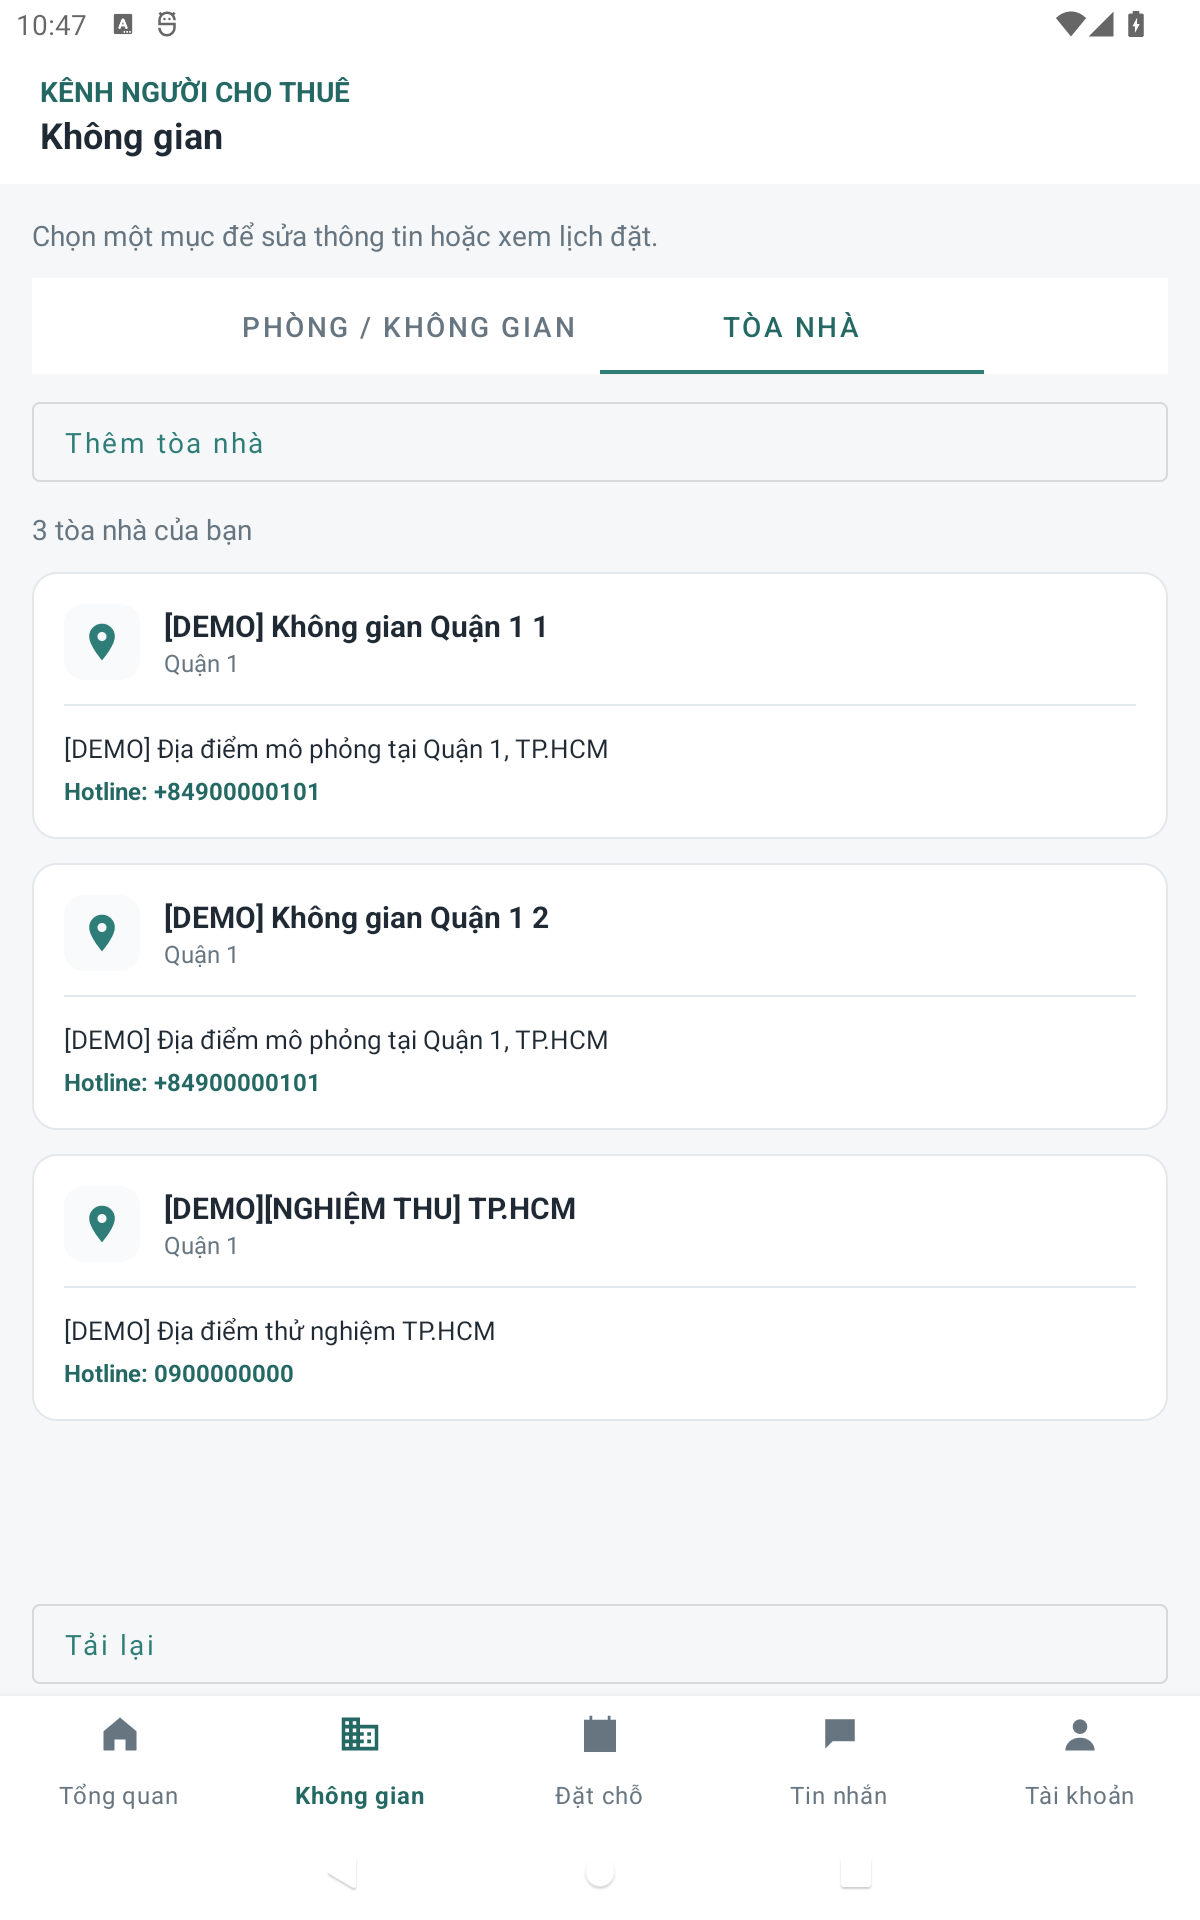
\includegraphics[height=0.40\textheight,width=\linewidth,keepaspectratio]{chapter5/members/host-tablet-buildings-portrait.png}\\[-1mm]
{\small (a) Tòa nhà của Host trên tablet}
\end{minipage}\hspace{0.05\linewidth}%
\begin{minipage}[t]{0.30\linewidth}\centering\vspace{0pt}
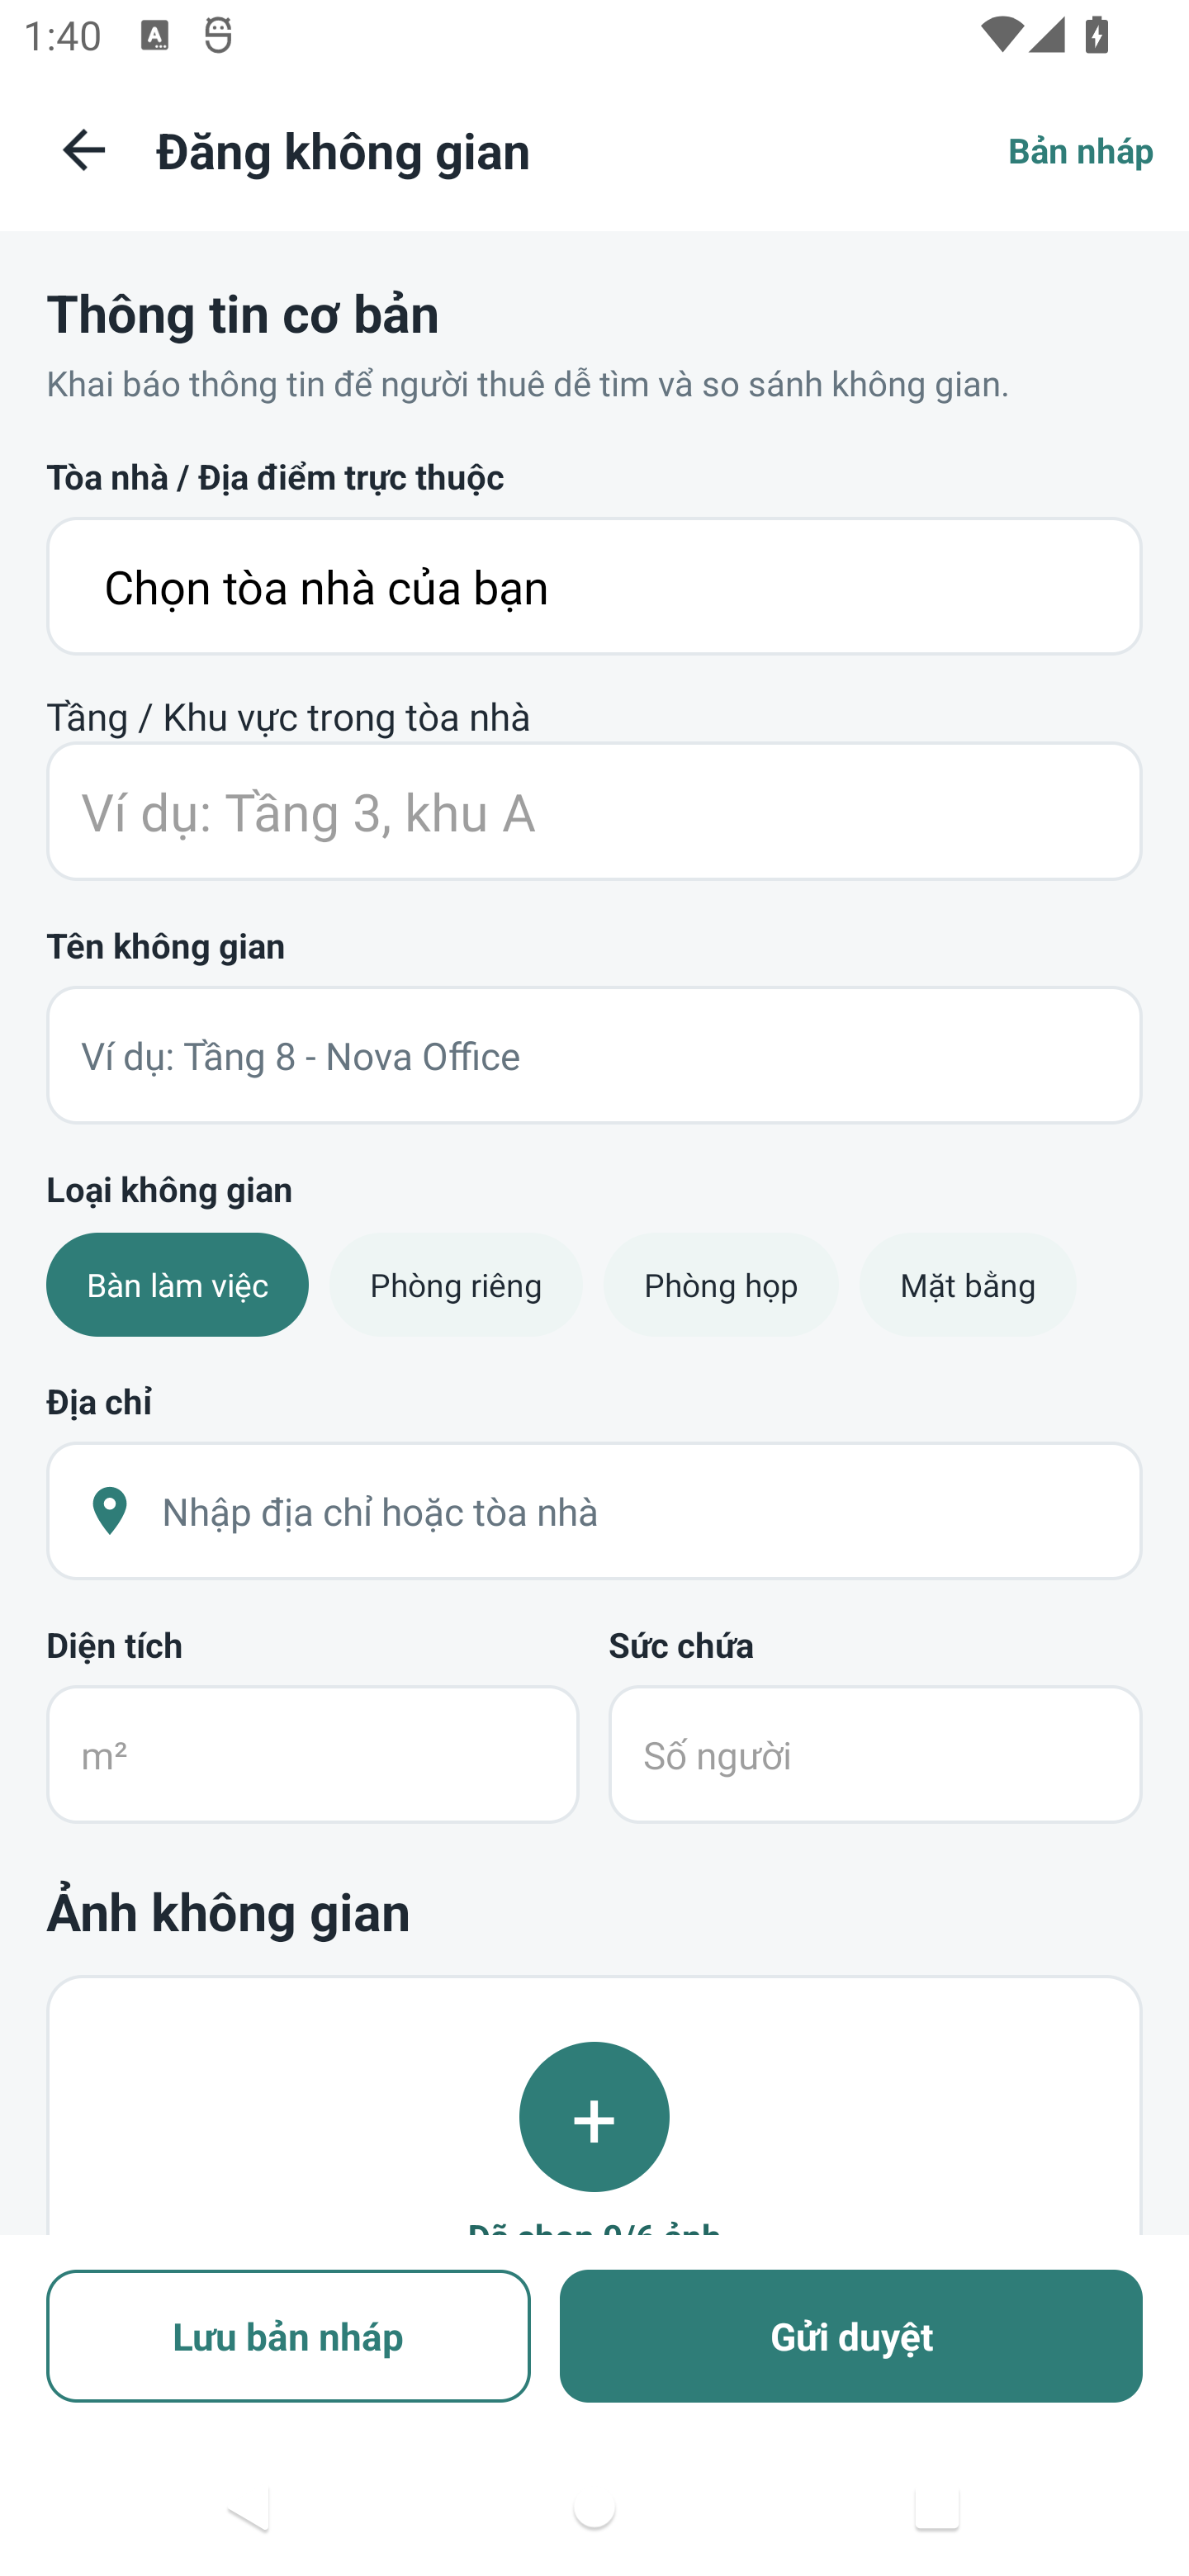
\includegraphics[height=0.40\textheight,width=\linewidth,keepaspectratio]{chapter5/final/host-create.png}\\[-1mm]
{\small (b) Biểu mẫu phòng trên điện thoại}
\end{minipage}
\caption{Quản lý địa điểm và khai báo không gian cho thuê}
\label{fig:actual-host-editor}
\end{figure}

Màn tổng quan ở Hình~\ref{fig:actual-host-overview} tổng hợp số không gian, tin chờ xét duyệt, phòng đang hiển thị và yêu cầu thuê của tài khoản hiện tại. Host chuyển từ các chỉ số này tới danh sách tương ứng. Số liệu được tính trên phòng và booking thuộc Host; phiên đang chờ thanh toán được phân biệt với lượt đã xác nhận.

\begin{figure}[!htbp]\centering
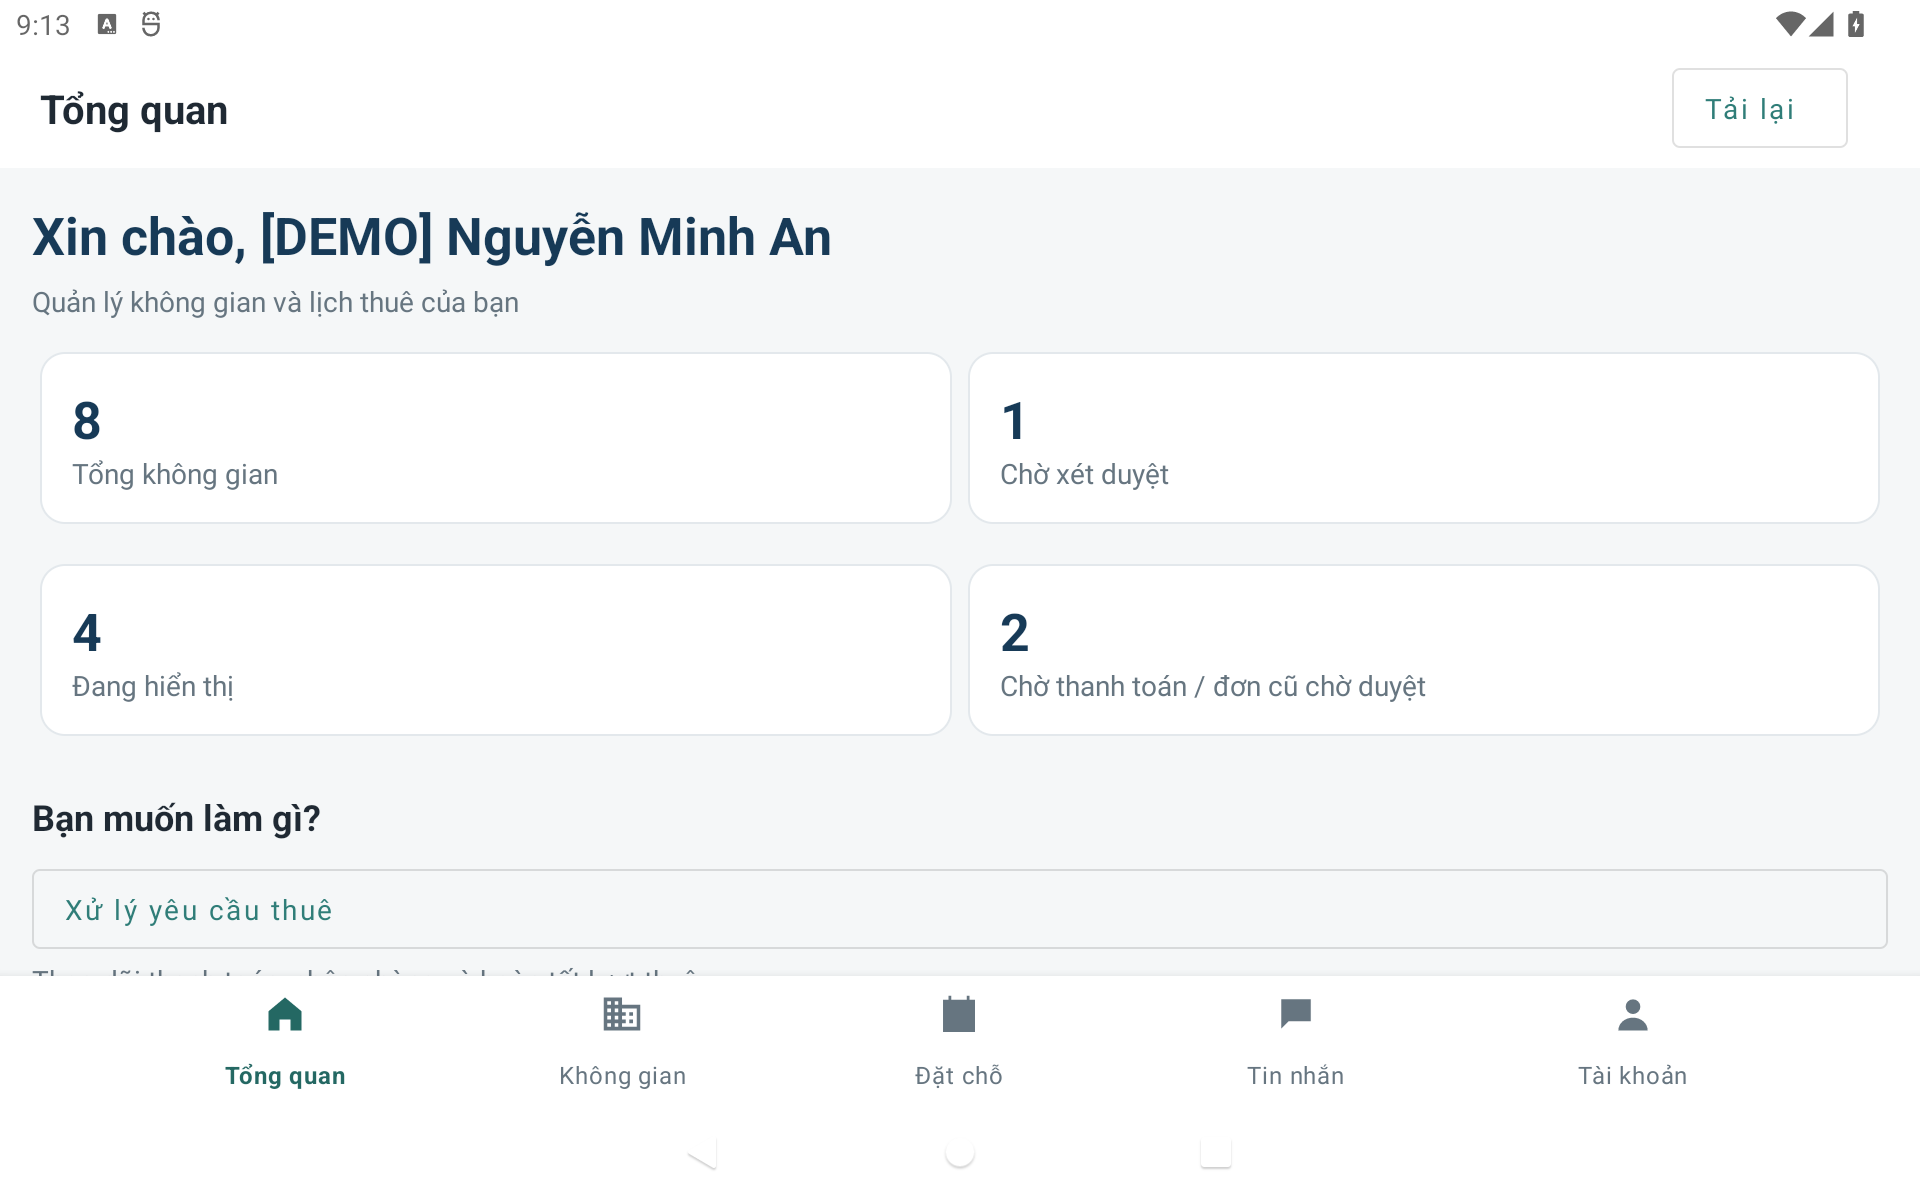
\includegraphics[width=0.96\linewidth]{chapter5/members/host-tablet-overview-landscape.png}
\caption{Tổng quan quản lý không gian của Host trên tablet}
\label{fig:actual-host-overview}
\end{figure}

Phòng lưu vào \texttt{rooms}, gắn Building và owner UID. Host chọn thuê giờ hoặc tháng/quý, khai báo giá, lịch hoạt động, ngày khóa và khoảng khóa; cấu hình ảnh giới hạn sáu tệp. HostViewModel tải ảnh qua Cloudinary trước khi ghi URL. Bản nháp và tin chờ duyệt có trạng thái riêng; quyền Host không thay thế quyết định duyệt từng bài đăng. Việc đổi chế độ hoặc lịch chịu kiểm tra các booking còn giữ chỗ để không làm sai kỳ thuê đã có.

\begin{figure}[!htbp]\centering
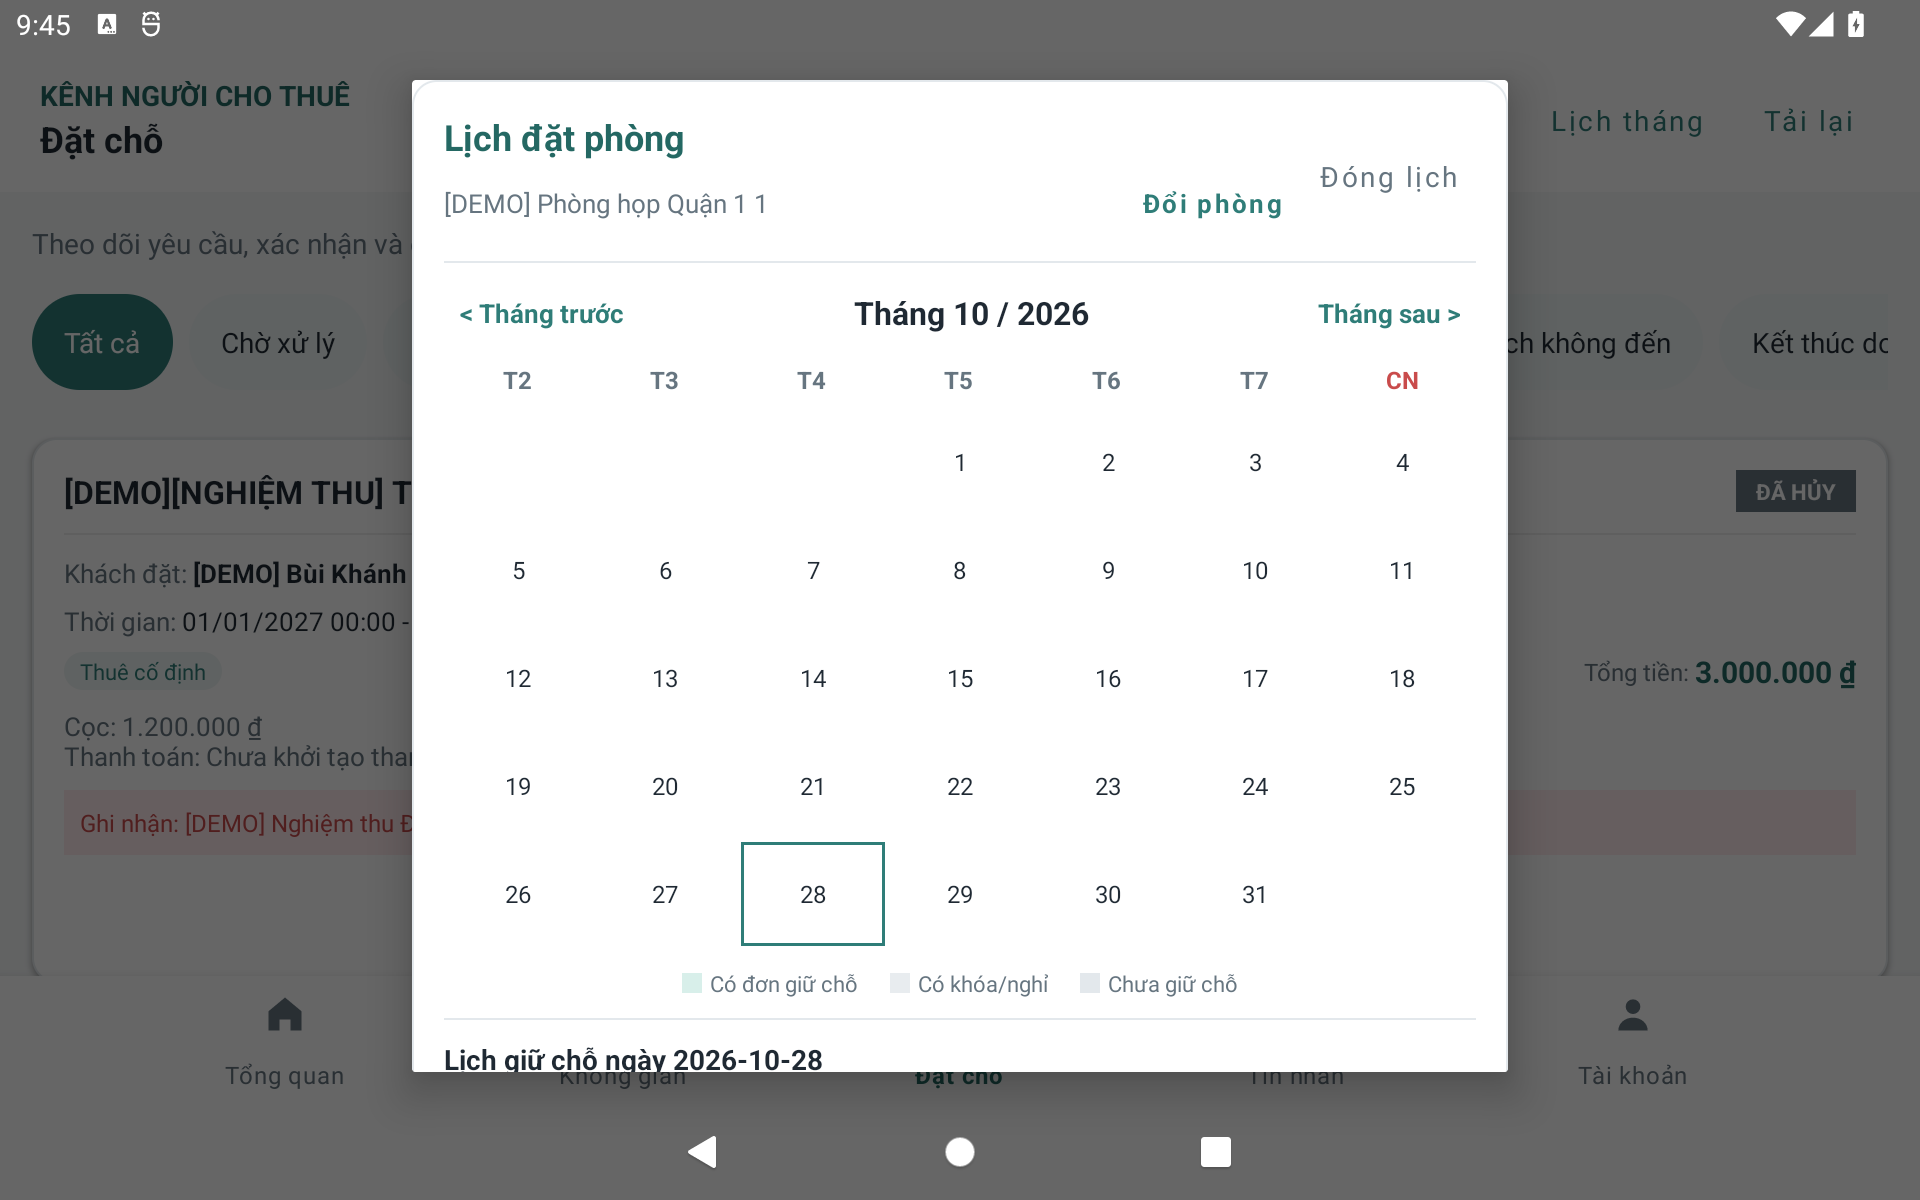
\includegraphics[width=0.96\linewidth]{chapter5/members/host-tablet-calendar-landscape.png}
\caption{Lịch đặt phòng theo tháng trong kênh Host}
\label{fig:actual-host-calendar}
\end{figure}
\FloatBarrier

Danh sách không gian phân biệt trạng thái xét duyệt với trạng thái hiển thị. Lịch tại Hình~\ref{fig:actual-host-calendar} tổng hợp khoảng giữ chỗ, ngày khóa và cho xem chi tiết theo ngày. Host theo dõi booking đã thanh toán, ghi nhận khách đến trong kỳ thuê, hoàn tất hoặc ghi nhận không đến theo điều kiện nghiệp vụ. Hồ sơ minh chứng LOCATION/PHOTOS và phản hồi báo cáo được xử lý tại các màn riêng.
